\chapter{Zielspezifikation ( 5 \%)}

Wie das letzte Kapitel gezeigt hat,
bringen bisherige Systeme diverse Probleme mit sich.
Da diese nicht oder nur schwer innerhalb dieser Systeme l\"osbar sind,
soll ein neues System geschafen werden.

Dieses Kapitel soll die entsprechenden Ziele qualitativ und quantitativ festlegen.


% tests in sektionen mit angeben

% zeitanforderungen ?!

% funktional, tests, szstemanforderunge? bessereer name
% abgrenzungen

%Was soll konkret gelöst werden. Hierzu gehören u.a.
%    -    Anforderungskatalog
%    -    Use-Cases
%    -    Pflichtenheft
%    -    Testkriterien
%    -    ... 


\begin{verbatim}
- funktional + use-cases
- testkriterien
-
\end{verbatim}


\section{Systemanforderungen}



- ausfallsicherheit bei absturz/beendigung
  von systemkomponenten
- standardschnittstellen fuer den datenbankzugriff
- grundlegende erweiterbarkeit

% kann/soll kriterien
\section{Funktionenale Anforderungen}
% evtl incl use-cases
\subsection{Funktions\"uberblick}
\begin{verbatim}

- einzelnen komponenten
  - auftragseingang
  - aftragsvorbereitung
  - auftragsabarbeitung
  - schritte durchlaufen

- schrittypen durchfuehren
 - prozess
 - python ?
 - scm



- projekt verwalten -> kann

- annahme/generieren von aufrtraegen
  - matrix mit werten -> muss

- erstellung/management von arbeitspacketen
  - von matrix
- abarbeitung von arbeitspacketen
  - scm
  - prozesse
- analyse von
  - zeitserien ueber projekte
  - auftraegen
  - arbeitspackete

  - ext analyse sommer projekt
  - ext regressionsanalyse (theorie) ?
\end{verbatim}

\subsection{Use Cases}



\begin{figure}[ht]
  \centering
  \label{fig:use-case-muss}
  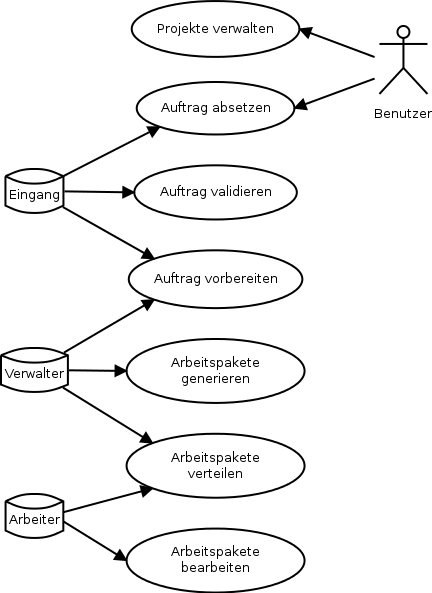
\includegraphics[width=0.7\textwidth]{imageinput/use-case-muss.png}
  \caption{\"Ubersicht Use-Cases - Kern}
\end{figure}


\begin{verbatim}
- build achsen ??

- extensions
  - regressionstest
  - testanalyse

- alte usecases
  - junitxml beispiel
  - stdout beispiel

- neue use-cases
  - workdir diff/tarball
  - auswertung zeitserien <addon>
  - datenanalyse beispiel sommer <addon>
\end{verbatim}


\section{rahmenbed}

\subsection{konkr}?
- testen notwendig
- das system selber ci unterziehen

\subsection{feststellung}
 - regeln


\section{Testkriterien}
\subsection{Unit Tests}

Unittests werden verwendet um die kleinsten Komponenten des Systems zu testen.
Durch ihre starke Koppelung an Implementation und Entwurf,
sind die nicht w\"ahrend der Kriterienfindung noch nicht n\"aher bestimmbar.

Sie ergeben ich im Entwurf und in der nachfolgenden Implementation.

\subsection{Funktionale Tests}

Funktionale Tests testen einzelne funktionale Komponenten des Systems.
Daher entsprechen sie Grob den funktionalen Anforderungen und Use-cases.
%XXX: mehr text

\subsection{Systemtests}

Systemtests testen Kombinationen von funktionalen Komponenten sowie das Komplettsystem.
Im Rahmen dieser Arbeit werden 3 Systemtests definiert.


\begin{description}
  \dhitem[Komponentendurchlauf]
    soll anhand des ausf\"uhrens der einzelnen funktionalen Komponenten
    aufzeigen, ob das Zusammenspiel der Komponenten
    grunds\"atzlich funkioniert
  \dhitem[Komplettstystem]
    soll das komplette CI-System auf einer Testdatenbank starten
    und seine Funktion sicherstellen
  \dhitem[Beispiel Datenanalyse]
    soll die Funktion der Beispielerweiterung f\"ur Datenanalyse sicherstellen
\end{description}

\subsection{Manuelle Tests}

Die manuellen Tests werden alle Tests umfassen,
deren Umsetzung als automatisches Programm erfahrungsgem\"ass zeitaufwendig,
fehleranf\"allig und/oder umfangreich sind.


\begin{description}
  \dhitem[Zeitverhalten]
    Beobachtung und Analyse des Zeitveraltens bei wachstender Datenmenge und Auftragsgr\"osse
  \dhitem[Raceverhalten]
    %XXX: besserer name als race?
    XXX
  \dhitem[Verhalten bei Systemfehler]
    \"Uberpr\"ufung des Verhaltens beim Absturz von Teilkomponenten
  \dhitem[Grosse Datenanalyse]
    Testen der exemplarischen Erweiterungen mit Datenmengen und Aufgaben
    die den Rahmen eines automatischen Tests Sprengen
\end{description}

\section{Zusammenfassung}

% zusammenfassung 
%   - im wesentlichen soll \ldots. prototypisch & exemplarisch
%   anhand .. soll ein loesungskonz vorgestellt werden
